\section*{Data-Parallel Execution Model}
The execution is SPMD, with each thread using unique coordinates
to access some region of the data-structure. A grid is a 3D-array
of blocks and a block is a 3D array of threads.

Each block has a 3-vector \texttt{blockIdx}, and each thread has
a 3-vector \texttt{threadIdx}, the components having identifiers
\texttt{x}, \texttt{y}, \texttt{z}. dimensions of each block and each
grid can be specified using variables of type \texttt{dim3}. If
scalar dimension specifiers are used (e.g. \texttt{int}), then
the \texttt{x} dimension is set to the scalar value while
the \texttt{y} and \texttt{z} are set to \texttt{1}. A grid
can have higher dimensionality then its blocks.

It might be a good practice to assign indices such that the largest
of the dimensions comes first, e.g.
\begin{minted}
{c}
dim3 dimBlock(2, 2, 1);
dim3 dimGrid(4, 2, 2);
KernelFunction<<<dimGrid, dimBlock>>>(...);
\end{minted}

This works better when mapping thread coordinates into data indices
in accessing multidimensional arrays.

NVIDIA GPUs in 2012 could support up to 1024 threads per block with
flexibility in how one can index them.

\subsection*{Mapping Threads To Multidimensional Data}
The programmer needs to think about the dimensionality of the grid
and blocks based on the nature of the data in consideration. E.g.
an image is a 2D grid of values. If the image is greyscale, then
we can do with a representation that takes a scalar value per pixel.

So, if the resolution of our image is $76\times 62$, we could create
a grid using $16\times 16$ blocks, and let the grid be $5\times 4$
blocks. $16\times 16$ is a typical choice of block dimensions for
2D data structures. In this example, we are allocating $80\times 64$
threads to process $76\times 62$ pixels.

To avoid wasteful computations, there should be a conditional guard
so that spawned threads in the grid that do not have pixel values to
work with do not do any computations, like was done in the vector
addition example, wherein four 256-thread blocks were spawned to
deal with a vector of length 1000.

If you have been provided with parameters for a 2D array, e.g. the
dimensions $m\times n$ for the image, then you can use something
like this two spawn a grid for processing the image.
\begin{minted}
{c}
    dim3 dimBlock(ceil(n/16.0), ceil(m/16.0));
    dim3 dimGrid(16, 16, 1);
    pictureKernel<<<dimGrid, dimBlock>>>(d_Pin, d_Pout, n, m);
\end{minted}

So, here's the important bit. We have a global memory pointer
\texttt{d\_Pin} for our input data. As of 2012, CUDA C is based on
ANSI C, which requires the number of rows and columns in 2D arrays
to be known at compile time, which spells doom for most of our
dynamically allocated datastructures. So, the programmer has to
explicitly flatten the tensor to an equivalent 1D array.

The most up to date documents on NVIDIA are on C++. The C documents
are 2010-ish old.The CUDA 11.0 guides on programming and best
practices are exclusive to C++.

Checking C99 compatibility would require some testing. For now, all
I need to know is that C arrays are stored in row-major order.

The following listing shows an example of a CUDA code for matrix
multiplication for square matrices
\begin{code}
\inputminted[samepage=false, breaklines, linenos]{c}{../codes/matrixAdd/matrixMul.cu}
\label{lst:matrixMul}
\caption{Multiplication of square matrices}
\end{code}

\subsection*{Synchronization and Transparent Scalability}
In general one has to coordinate the execution of threads. CUDA allows
threads in the same block to coordinate using a barrier
synchronization function \texttt{\_\_syncthreads()}. All threads
in the calling block will be held until all threads reach the same
location in the program. I see potential deadlocks.

At the very least using this particular barrier synchronization
would allow different blocks to execute independent of each other.

\subsection*{Thread Scheduling and Latency Tolerance}
Thread scheduling depend on specific hardware implementations, A warp
is a unit of thread scheduling, typically 32 threads, but is not
defined in the CUDA specification. A streaming multiprocessor
executes all threads in a WARP in a SIMD fashion - all threads in a
warp will have the same execution timing.

In general, there are fewer streaming processors (SP) per SM than
the number of threads assigned to each SM; a scheduler is involved
in the execution of all the warps assigned to an SM. By having
more warps per SM than what the underlying hardware can execute at
a time, CUDA processors efficiently execute long latency operations
such as global memory accesses - context switching. Another resident
warp that is not scheduled is then scheduled and the previously
scheduled warp, that is waiting for the completion of a long latency
operation is queued.

Examples of long latency operations include pipelined FP arithmetic,
branch instructions etc. \textit{Note that warp scheduling has zero-overhead when switching to another ready warp.}

\subsection*{SIMT and Warp-Level Primitives}
I came across a nice blog post by NVIDIA on warp-level primitives.
The question that I had been trying to address was ``is it safe to
remove \texttt{\_\_syncthreads()} when the block size is the same as
the device warp size?". The answer is no. There can be divergent
control flow between threads in the same warp. The simplest
example is when checking boundary conditions when working with
tensors/tensor-like data structures.

While GPU computing is usually defined as SIMD (Single Instruction
Multiple Thread), the classification SIMD in the context of Flynn's
taxonomy is usually reserved for vector architecture, i.e. a
scalar thread issues vector instructions, and the exact same
instruction is applied across many data elements.

SIMT (Single Instruction Multiple Thread) is a more appropriate
classification for GPUs, even at the level of a single warp. Each
thread has access to its own registers and can load and store from
divergent addresses and follow different control paths.

It is possible to achieve even higher performance by using warp-level
primitives and exploiting the flexibility provided by this SIMT
architecture.

A consequence of this is that we can have cooperative groups
collectives, e.g. accumulating the sum of values in all threads
into a single thread (analogous to \texttt{MPI\_Reduce}).

\begin{minted}
    {c}
    #define FULL_MASK 0xffffffff
    for (int offset = 0x10; offset > 0; offset /= 2)
        val += __shfl_down_sync(FULL_MASK, val, offset); 
\end{minted}

The above code performs a tree-reduction to compute the sum of
the \texttt{val} variable held by each thread in a warp. See figure
\ref{fig:figures-shfldown-png}

\begin{figure}[h]
    \centering
    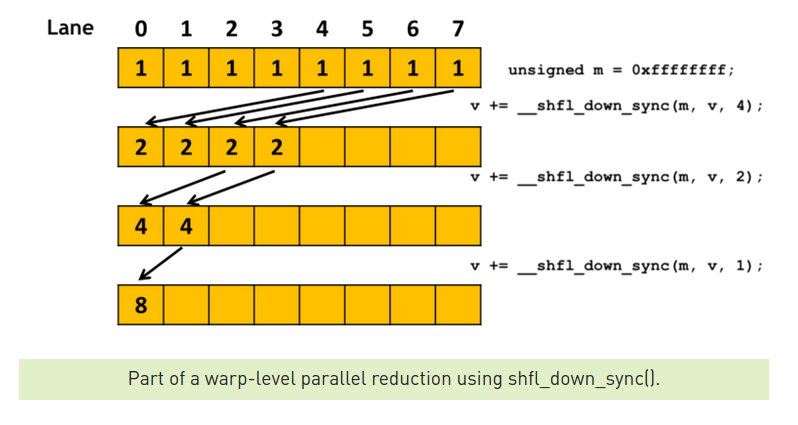
\includegraphics[width=0.8\textwidth]{figures/shfldown.png}
    \caption{Warp-level parallel reduction (taken from NVIDIA's blog)}
    \label{fig:figures-shfldown-png}
\end{figure}

(TODO: document some warp-level primitives)
